\chapter{Introduction}
\label{cha:Introduction}

\section{Motivation}
\label{sec:Motivation}
\subsection{Path Planning in Robotics}
In the field of robotics the path planning of an industrial robot can be programmed as a fixed list of movements to be executed. This has multiple drawbacks as for every change in the enviroment the robot needs to manually be reprogrammed.\\
But what if this robot is equipped with a camera that detects the shape of objects in the robots enviroment. This would give a set of objects at certain positions, a robot arm in a starting position and a target where the robots endeffector needs to work. If then this puzzle would be solved, the robot could be directed in a different way each time without the actual need to access its software.


\subsection{Geometric Riddles in Gaming}
Solving geometric riddles is an amazingly fun task for a human. This is the reason many games simply consists of such riddles ranking from easy to hard in difficulty. But even the easiest riddle for a human proposes a big challenge for a simple algorithm that searches trough the possible ways of solving it. Even more complicated is the generation of such riddles. Even for the human brain this task can be exceedingly stressful.\\
 Now, if there would be a possibility to check if such a riddle has a solution, there would be the option to generate them randomly and check for feasibility. This would cast off the necessity for the developers to manually create each riddle. Also the consumers, in this case the players, would have a endlessly stream of new and different riddles to solve.


\section{Idea}
\label{sec:Idea}
For simplification purposes the algorithms work on two dimensional object displacement problems. The following riddles shall provide simple examples of the problem:\\

\begin{figure}[h]\centering
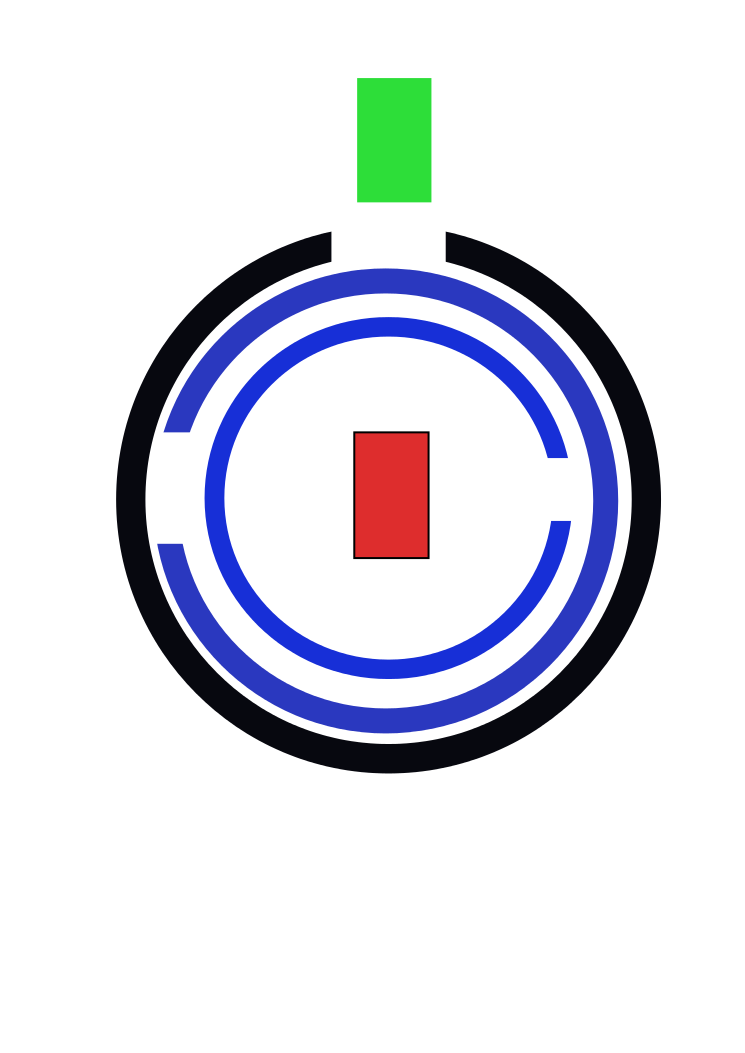
\includegraphics[scale=0.1]{circleRiddle.png}
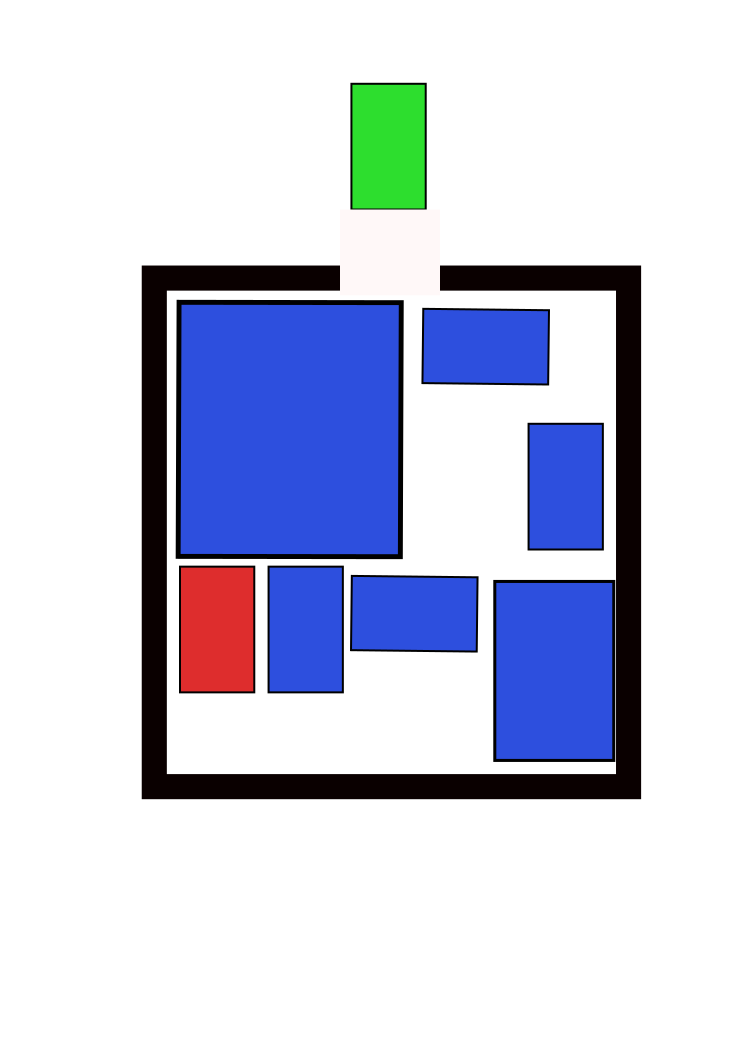
\includegraphics[scale=0.1]{boxRiddle.png}
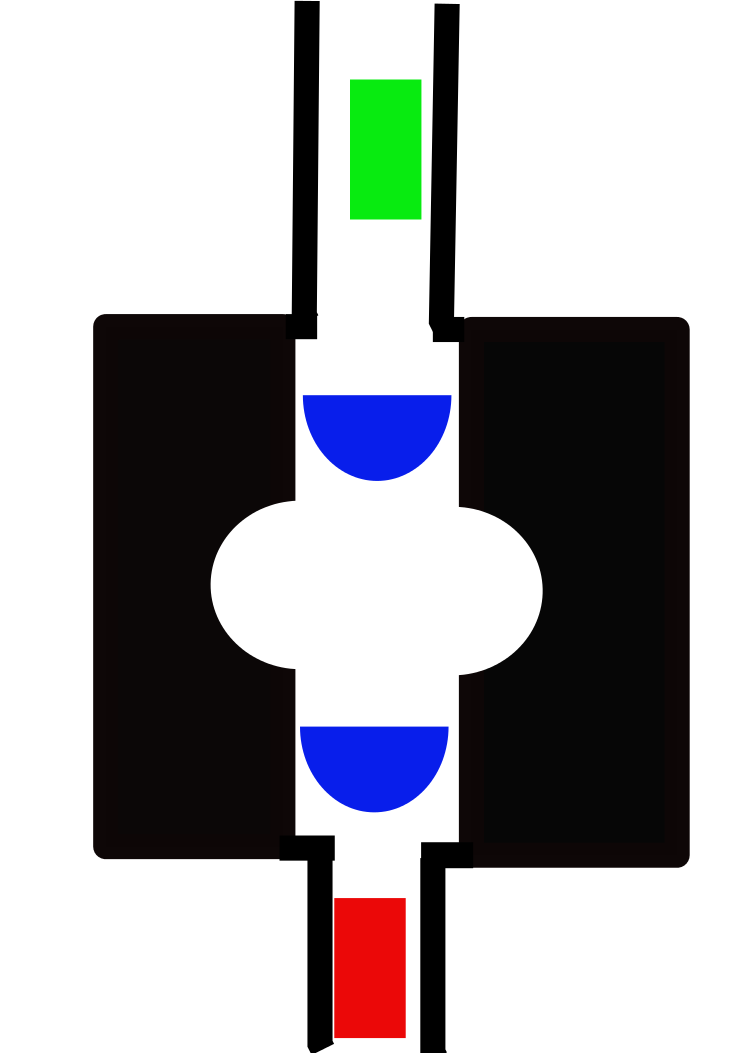
\includegraphics[scale=0.1]{mixedRiddle.png}
\caption{riddle 1 with circles , riddle 2 with boxes , riddle 3 with 2 half-circles}
\end{figure}

The riddle is solved, if the red box matches the green one. Blue objects are movable and black ones are stationary. The stationary ones will be referred to as rims hereafter.\\
As a human the way of finding solutions is quite obvious. The first riddle is solved by rotating the blue objects, the second through translation. The third needs both ways to be solved.\\
If the riddle should be solved with an algorithm, each objects collsision with the other objects and the rim has to be accounted for. Also the questions how to express the current position of an object consisting of its corner points, position (x,y) and rotation ($\phi$) needs to be answered. A first idea would be to 
\begin{enumerate}
\item Generate all valid configurations per object in regard to the stationary obstacles as a configuration space.
\item Create one collision space per object for collision with every other object. 
\item Substract the collision space from the configuration space to get a valid space in regard to all obstacles for one object.
\item Divide the space in cells and locate the valid ones.
\item Build a graph out of this starting position by adapting the space after each step.
\item Search in that graph to get a path from the  start to the target point.
\end{enumerate}

The target point would then be a simple configuration vector holding each position of each object. A user defined distance function beetween start and target point in that space can then be used as heuristic in the graph search, e.g. $h(start,target) = || ( x_{start} -  x_{target} , y_{start} - y_{target} ) ||$ .


\section{State of the Art}
In the following part a short overview of the current state of the art algorithms in path planning and collision detecten is given, as these two are the major fields necessary for implementing the final algorithm to solve a geometric riddle. Also a short look is taken into the way complete solutions are present in the possible fields of applications.
\subsection{Path Planning}
The correct answer to the question "Which algorithm is the best for finding the path from start to target" is not as easy as one might suspect. 
It depends on many factors including which structure one searches on ( e.g. graph, net, tree ), what knowledge there is about the current position ( e.g. distance to target ) and what result is needed ( shortest path, "good" path, existence of a path ).\\
For this work the focus is on an algorithm working on a graph with non-negativ edges, an absolute knowledge of the position of the target and the current in a two dimensional coordinate system and a need for a "good" path, not necessarily the shortest. Given these conditions, A$^\star$ \cite{ComputerScience} is a valid choice. It is a widely used algorithm which calculates a "good" path, not a perfect one. How good the path is depends heavily on the heuristic used. In the given example this would be a weighted sum of the distance traveled in steps plus the absolute distance to the target.\\
Another choice could be Dijkstra's algorithm \cite{ComputerScience} itself which is basically A$^\star$ with the heuristic set to constant zero. This would return the shortest path for all calculations. For the named applications from \ref{sec:Motivation} the algorithm should be fast, more than precise, thus A$^\star$ is the better choice.\\
Normally A$^\star$ would have access to the complete graph to calculate the best way to the target. As this is not the case an adapted form called RTA$^\star$ \cite{rta} is used. It introduces a lookahead depth for A$^\star$, telling the algorithm to only make a choice using the information gathered by the nodes in the rims to a certain depth of the graph. In this implementation, this value will be set to one, as only one object is moved in one direction at a time, thus generating the graph while searching step by step. The drawback is, that the quality of the final path is lower for lower lookahead depths.\\
Another idea would be to use a potential field method which is quite commen in mobile robotics. This method lays out a grid and for each point a sum is calculated over the repulsive vectors of the obstacles and the attractive target vector \cite{hwang1992potential}. 
It should be noted though that the algorithm for pathplanning is exchangable. Depending on the choosen method the amount of work needed to adapt the algorithm varies.

\subsection{Collision Detection}
Collision detection in computer science has its home in simulations and computer games as it has in robotics. In this case the focus lies on the way computer games solve collision detection without looking into physical problems that would arise with it.\\
There are a number of ways this has been solved. In a case where there are not too many objects needed to be considered, pairwise checking is an option. Depending on how the objects are represented, they need to be checked for collision for every step taken. A system was divised by letting only small movements happen in beetween steps \cite{pairwise} to eliminate checking for all objects. Another way around this is to bound objects that lie in a certain proximity of each other together in spheres, where they are only checked in pairs if the spheres containing the objects collide \cite{sphere}.\\
Also there is a difference in checking if a collision happened, or if it is about to happen. The first option is easy to calculate, because all that is needed is the current position of the objects concerned. If there is the need to calculate the collision beforehand, some information about the movement is needed. As time is not a factor, movement in this scope only refers to position changes in the direction of a vector. Therefore it is possible to calculate the next collision in the direction of the vector to obtain the allowed moving distance.\\
One way is to start building a spacial binary tree starting from the object, partioning the space along the direction of the movement. Until a given spacial size of an end node is reached ( e.g. the bounding box of the moving object) or a obstacle is in the node, the tree keeps on growing. The node directly in front of the last obstacle node would then be choosen as the last safe position to move to. This approach was used in the context of mobile robotic pathplanning \cite{binTree}.\\
The SWIFT++ algorithm \cite{swift} uses bounding boxes around all object. Then a collision check of this bounding box with other bounding boxes in the area  is done to remove unnecessary checks. After that simple pairwise checking using the Minkowski sum is done. As this is designed to work with a time axis, steps are supposed to be small, thus it does not suit the needs of this work entirely.\\
What is needed to prevent a collision, is the distance to the next obstacle. In a work by Ming C. Lin the distance is calculated using either convex polyhedra and a check for bounds or algreabic functions and check for crossings \cite{collision}. In his work this was used to determine if a collision occured, but using the principle ideas one can also calculate the distance to the next obstacle.\\


\subsection{Applications}
The easiest solution in path planning for industrial robots is to hard-code the correct path. This is mostly done by setting a number of safe points on the path from start to target to avoid a collision. As a matter of fact, this is a good solution for processing objects where only one simple step for a large quantity is needed. In this scenario only few recalibrations are needed. But if the processed objects change more often, each time the machinist needs to recalibrate the robot. \\
There are already algorithms in work adressing this problem. One algorithm indroduced in the proceedings of IEEE from April 2000 uses Lazy PRM to calculate a collision free path on a grid starting with perfekt path and recalculating edges that include collisions \cite{lazyPRM}.\\
Earlier work suggests using an approach with local potential field optimization to obtain a good path to the target \cite{potField}.\\
The drawback for both algorithms is, that only static obstacles are taken into account. If the algorithm introduced in this work is used to calculate a path, multiple movable objects would be allowed.\\
\newline
Assembly planning describes the process of planning the movements for $n$ objects to fit in $n$ target positions, such that a final object  is constructed out of smaller parts. The standart approach uses the finished product as a starting point, trying to find movements to disassemble it into smaller parts. There are multiple algorithms in place to achieve such a plan. A study from Université Libre de Bruxelles suggests using an ordering genetic algorithm in a way, that the sequence of movements is evolved through mutation or crossover and validated until a solution is reached \cite{genAssembly}. Another approach would be using motion space representation, where each point in space represents a possible motion of a subassembly \cite{motionAssembly}. A special interest lies on a geometrical approach to assembly planning \cite{geoAssembly}, as the representation of objects is very close, if not equal in some cases, to the objects in this work. Even though another way of planning the path by decomposing the finished object is presented, it seems possible to adapt the problem of assembly planning to a generic riddle with multiple main objects. As the algorithm in this work is written to compute a path for one main object this is not in the scope of this thesis.\\
\newline
The automated creation of geometric riddles in computer games is a process widely used in the gaming industry. Not only riddles, whole characters and worlds are created at random.
One of the first famous games making use of that concept was Nethack \cite{nethack}. It featured randomized enemy characters in randomized levels. This concept is still in use in todays products. The problem is, that this randomized content is created reversely. For example starting with a valid riddle/ level and then  doing only steps from a certain predetermined set of valid transformations one would reach a randomized mutation which can be used as new content.\\
A newer example is that of Galactic Arms Race, a game using an algorithm called cgNEAT \cite{cgNEAT}. The main idea of this algorithm is to evolve from existing game content in a matter similar to the evolution of species in biology. This is a huge improvement in contrary to the pseudo-random generated content in older games. But still it needs an initial game content to start from.\\
The way one could create content with the algorithms in this work is very different. There would be the option to place "totally" random objects into the riddle and afterwards check for the existence of a solution. "Totally" is relativ because there is still the need to look at the given properties of the riddle. For example if the riddles total space should only be 16x16 units big, putting an object the size of 1x30 units in would not be possible.

